\documentclass{article}
\usepackage{enumerate}
\usepackage{amsmath}
\usepackage{amssymb}
\usepackage{graphicx}
\usepackage{subfigure}
\usepackage{geometry}
\usepackage{color}
\usepackage{bm}
\usepackage{indentfirst}
\usepackage{array}
\usepackage{multirow}
\usepackage{diagbox}

\begin{document}

\vspace*{0.25cm}

\hrulefill

\thispagestyle{empty}

\begin{center}
\begin{large}
\sc{UM--SJTU Joint Institute \vspace{0.3em} \\ Physics Laboratory \\(VE215)}
\end{large}

\hrulefill

\vspace*{5cm}
\begin{Large}
\sc{{Laboratory Report}}
\end{Large}

\vspace{2em}

\begin{large}
\sc{{Exercise 5
\vspace{0.5em}

Filter Lab
}}
\end{large}
\end{center}


\vfill

\begin{table}[h!]
\flushleft
\begin{tabular}{lll}
Name: Yihao Liu \hspace*{2em}&
ID: 515370910207\hspace*{2em}\\


\\

Date: 17 Nov 2016 

\end{tabular}
\end{table}

\hfill
\begin{tiny}
[rev. 1.0]
\end{tiny}
\newpage


\section{Goal}
\begin{enumerate}
\item
Learn about four types of filters – Low-Pass, High-Pass, Band-Pass, and Band-reject.
\item
Learn about transfer functions.
\item
Predict the theoretical result and make comparison with lab data.
\end{enumerate}

\section{Introduction}

\subsection{Filter}
Filters are everywhere in our lives. The circuits built to operate on signals usually apply filters. For example, telephone lines pass the sounds at frequencies between about 100Hz and 3kHz and practically blocks all other frequencies.

\subsection{Transfer function}
Mathematically, the transfer function is used to analyze what the circuit did to the signal:

$$Transfer\ function=\frac{Output\ signal}{Input\ signal}$$

This function can also be expressed as

$$H(\omega)=\frac{V_{out}(\omega)}{V_{in}(\omega)}$$

The magnitude of the transfer function is called “voltage gain”, often measured as the ratio of the peak-to-peak (ppk) voltages:

$$|H(\omega)|=\left|\frac{V_{out}(\omega)}{V_{in}(\omega)}\right|=\frac{V_{out,ppk}(\omega)}{V_{in,ppk}(\omega)}$$

It is convenient to express and plot the magnitude of the transfer function on the logarithmic scale using decibels:

$$|H(\omega)|_{db}=20\cdot\log_10\left(\frac{V_{out,ppk}(\omega)}{V_{in,ppk}(\omega)}\right)$$

Since both ppk voltages are always positive, the transfer function magnitude is positive and thus can always be converted to decibels. The use of decibels allows us to review data over a broad range.

\newpage

\subsection{Types of filters}

\begin{figure}[!h]
	\centering
	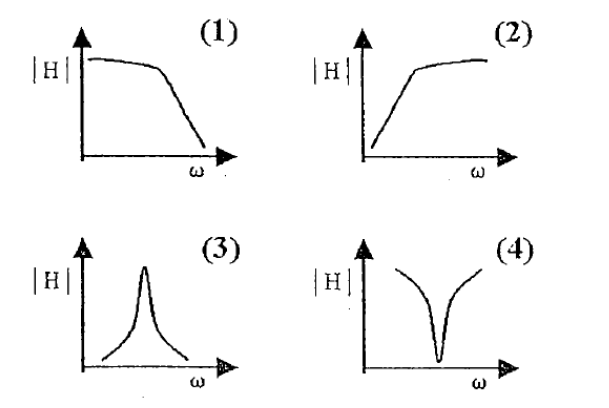
\includegraphics[width=12cm]{1.png}
	\label{fig-1}
\end{figure}

In the figure above are the four main families of filters:
(1): Low-Pass; (2): High-Pass; (3): Band-Pass; (4): Band-reject (also called band-stop or notch)

\begin{figure}[!h]
	\centering
	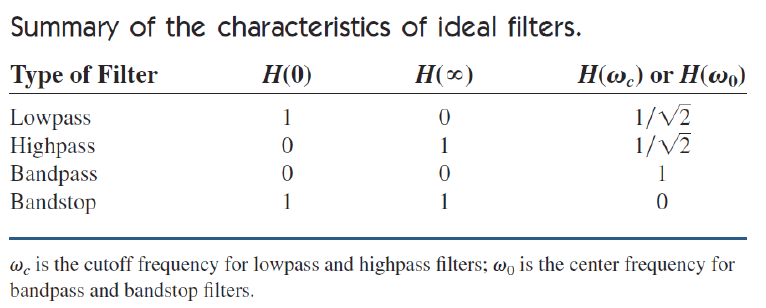
\includegraphics[width=12cm]{2.png}
	\label{fig-2}
\end{figure}

Filter circuits, which you are going to build in this lab, contain resistors, capacitors, and inductors. They are all passive filters.

\newpage

\subsection{High-Pass filter}

The high-pass filter we are going to build uses a capacitor and a resistor.

\begin{figure}[!h]
	\centering
	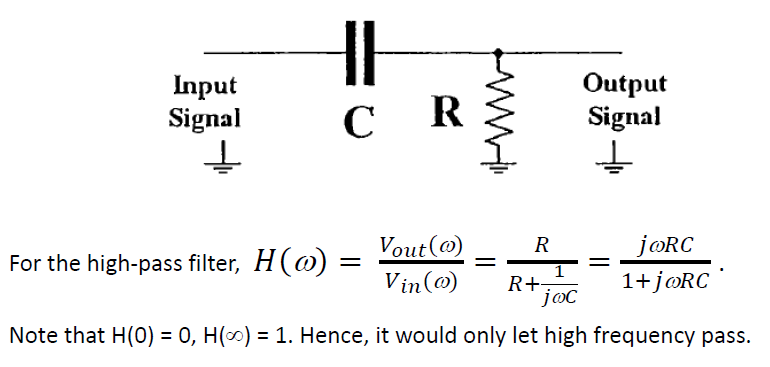
\includegraphics[width=12cm]{3.png}
	\label{fig-3}
\end{figure}

\subsection{Low-Pass filter}

The low-pass filter we are going to build uses a capacitor and a resistor.

\begin{figure}[!h]
	\centering
	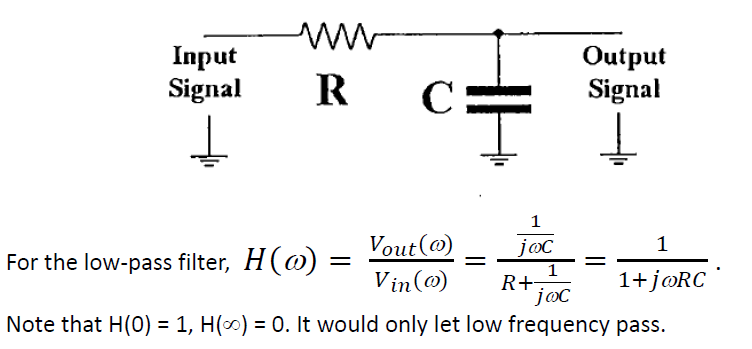
\includegraphics[width=12cm]{4.png}
	\label{fig-4}
\end{figure}

\subsection{Band-Pass filter}

The band-pass filter we are going to build uses a capacitor, an inductor and a resistor.

\begin{figure}[!h]
	\centering
	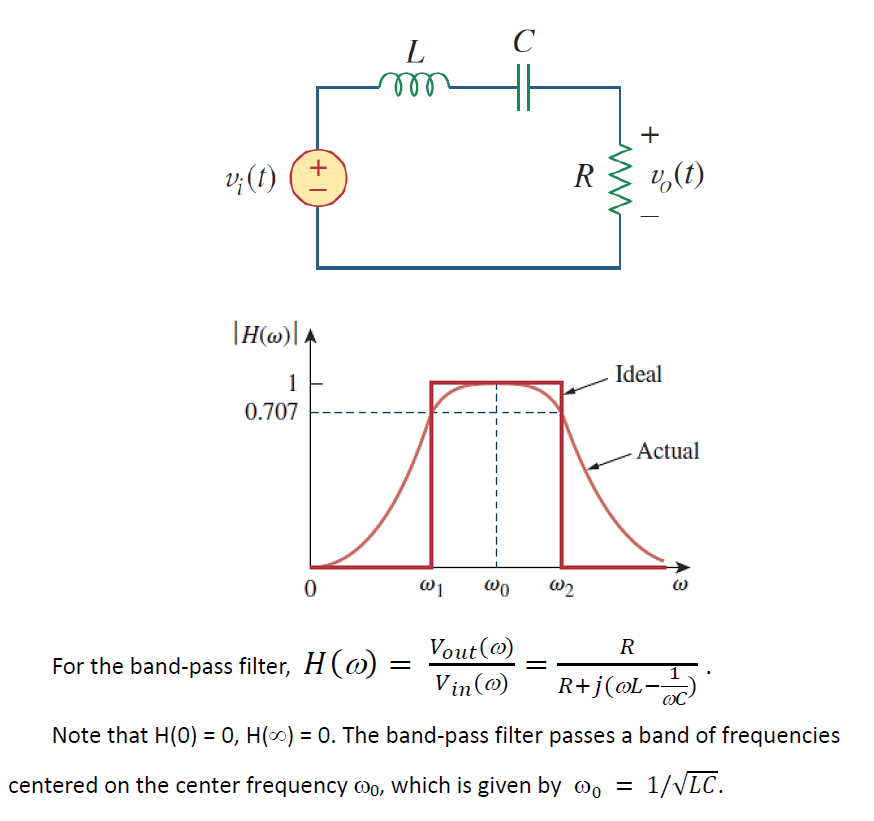
\includegraphics[width=12cm]{5.png}
	\label{fig-5}
\end{figure}

\newpage

\subsection{Band-Stop filter}

The band-stop filter we are going to build uses a capacitor, an inductor and a resistor.

\begin{figure}[!h]
	\centering
	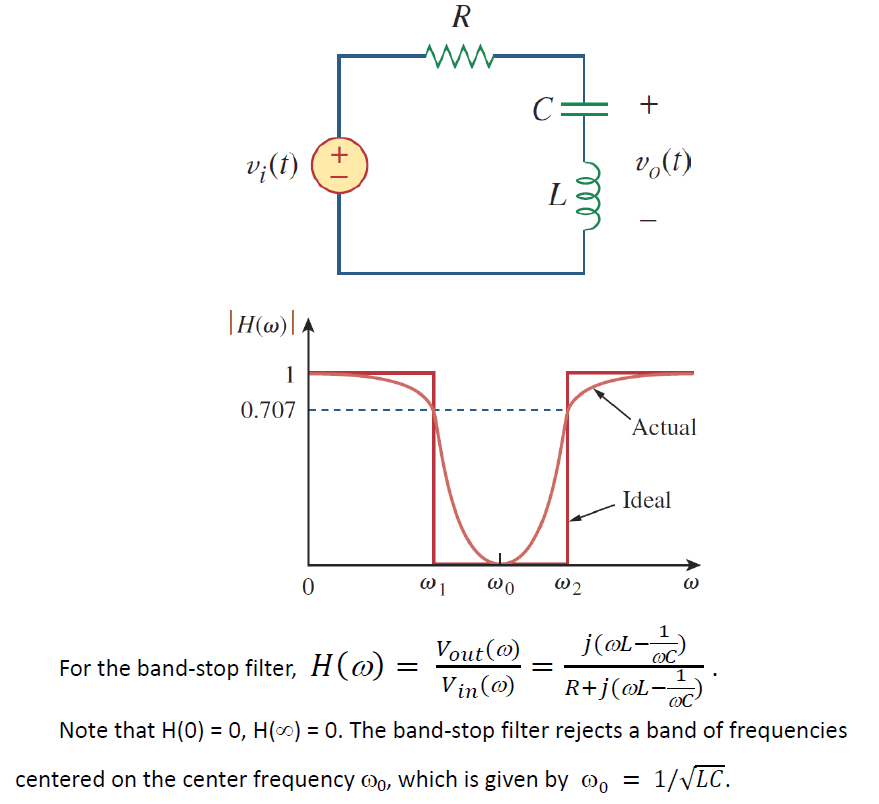
\includegraphics[width=12cm]{6.png}
	\label{fig-6}
\end{figure}

\newpage

\section{Results and Discussion}

\subsection{Low-pass Filter}

\begin{table}[!h]
\begin{center}
\begin{tabular}{|p{2cm}|p{2cm}|p{2cm}|p{2cm}|p{2cm}|p{2cm}|p{2cm}|}
\hline
Frequency & Input signal amplitude, Vppk & Output signal amplitude, Vppk & Transfer function magnitude & Expected transfer function magnitude & Transfer function magnitude, in dB & Expected transfer function magnitude, in dB \\
\hline
1000000Hz	&	4.80	&	0.024	&	0.005	&	0.002	&	-46.167	&	-55.806	\\
\hline
100000Hz	&	4.72	&	0.109	&	0.023	&	0.016	&	-32.730	&	-35.807	\\
\hline
50000Hz	&	4.68	&	0.208	&	0.044	&	0.032	&	-27.044	&	-29.790	\\
\hline
10000Hz	&	4.72	&	0.904	&	0.192	&	0.160	&	-14.355	&	-15.918	\\
\hline
5000Hz	&	4.72	&	1.680	&	0.356	&	0.308	&	-8.973	&	-10.219	\\
\hline
1000Hz	&	4.88	&	4.160	&	0.852	&	0.851	&	-1.387	&	-1.401	\\
\hline
500Hz	&	4.92	&	4.600	&	0.935	&	0.956	&	-0.584	&	-0.395	\\
\hline
\end{tabular}
\label{tab-low}
\end{center}
\end{table}


\subsection{High-pass Filter}

\begin{table}[!h]
\begin{center}
\begin{tabular}{|p{2cm}|p{2cm}|p{2cm}|p{2cm}|p{2cm}|p{2cm}|p{2cm}|}
\hline
Frequency & Input signal amplitude, Vppk & Output signal amplitude, Vppk & Transfer function magnitude & Expected transfer function magnitude & Transfer function magnitude, in dB & Expected transfer function magnitude, in dB \\
\hline
1000000Hz	&	4.76	&	4.720	&	0.992	&	1.000	&	-0.073	&	-0.000	\\
\hline
100000Hz	&	4.72	&	4.680	&	0.992	&	1.000	&	-0.074	&	-0.001	\\
\hline
50000Hz	&	4.68	&	4.600	&	0.983	&	0.999	&	-0.150	&	-0.005	\\
\hline
10000Hz	&	4.72	&	4.480	&	0.949	&	0.987	&	-0.453	&	-0.113	\\
\hline
5000Hz	&	4.72	&	4.240	&	0.898	&	0.951	&	-0.932	&	-0.434	\\
\hline
1000Hz	&	4.84	&	2.260	&	0.467	&	0.525	&	-6.615	&	-5.595	\\
\hline
500Hz	&	4.88	&	1.300	&	0.266	&	0.295	&	-11.490	&	-10.610	\\
\hline
100Hz	&	4.96	&	0.286	&	0.058	&	0.062	&	-24.782	&	-24.211	\\
\hline
\end{tabular}
\label{tab-high}
\end{center}
\end{table}


\subsection{Band-pass Filter}

\begin{table}[!h]
\begin{center}
\begin{tabular}{|p{2cm}|p{2cm}|p{2cm}|p{2cm}|p{2cm}|p{2cm}|p{2cm}|}
\hline
Frequency & Input signal amplitude, Vppk & Output signal amplitude, Vppk & Transfer function magnitude & Expected transfer function magnitude & Transfer function magnitude, in dB & Expected transfer function magnitude, in dB \\
\hline
1000000Hz	&	5.04	&	0.296	&	0.059	&	0.154	&	-24.623	&	-16.224	\\
\hline
500000Hz	&	5.00	&	1.290	&	0.258	&	0.299	&	-11.768	&	-10.498	\\
\hline
100000Hz	&	4.80	&	4.080	&	0.850	&	0.849	&	-1.412	&	-1.427	\\
\hline
50000Hz	&	4.72	&	4.440	&	0.941	&	0.961	&	-0.531	&	-0.345	\\
\hline
10000Hz	&	4.72	&	4.480	&	0.949	&	0.995	&	-0.453	&	-0.042	\\
\hline
1000Hz	&	4.84	&	2.280	&	0.471	&	0.527	&	-6.538	&	-5.570	\\
\hline
500Hz	&	4.88	&	1.320	&	0.270	&	0.295	&	-11.357	&	-10.602	\\
\hline
\end{tabular}
\label{tab-band_pass}
\end{center}
\end{table}


\subsection{Band-reject Filter}

\begin{table}[!h]
\begin{center}
\begin{tabular}{|p{2cm}|p{2cm}|p{2cm}|p{2cm}|p{2cm}|p{2cm}|p{2cm}|}
\hline
Frequency & Input signal amplitude, Vppk & Output signal amplitude, Vppk & Transfer function magnitude & Expected transfer function magnitude & Transfer function magnitude, in dB & Expected transfer function magnitude, in dB \\
\hline
1000000Hz	&	4.88	&	3.760	&	0.770	&	0.988	&	-2.265	&	-0.105	\\
\hline
500000Hz	&	4.96	&	4.840	&	0.976	&	0.954	&	-0.213	&	-0.406	\\
\hline
300000Hz	&	4.92	&	4.720	&	0.959	&	0.886	&	-0.360	&	-1.048	\\
\hline
200000Hz	&	4.84	&	4.120	&	0.851	&	0.786	&	-1.399	&	-2.091	\\
\hline
100000Hz	&	4.72	&	2.260	&	0.479	&	0.529	&	-6.397	&	-5.528	\\
\hline
50000Hz	&	4.68	&	1.320	&	0.282	&	0.276	&	-10.993	&	-11.172	\\
\hline
10000Hz	&	4.65	&	0.584	&	0.126	&	0.098	&	-18.021	&	-20.209	\\
\hline
5000Hz	&	4.68	&	1.480	&	0.316	&	0.280	&	-10.000	&	-11.044	\\
\hline
1000Hz	&	4.76	&	4.160	&	0.874	&	0.850	&	-1.170	&	-1.410	\\
\hline
500Hz	&	4.80	&	4.040	&	0.842	&	0.955	&	-1.497	&	-0.396	\\
\hline
\end{tabular}
\label{tab-band_reject}
\end{center}
\end{table}


\newpage

\section{Conclusion}
We learned about four types of filters – Low-Pass, High-Pass, Band-Pass, and Band-reject.\\
We learn about transfer functions.\\
We predicted the theoretical result and make comparison with lab data.

\section{Reference}
Lab 5 Manual.

\section{Pre-lab and Data sheet}

\end{document}